% =============================================================================
% P3A -- Privacidade 2: pôster (PT-BR)
% Formato: A1 retrato (594 x 841 mm), duas colunas, fonte Latin Modern.
% Figuras esperadas em out/: Fig1_PT.pdf, Fig2_PT.pdf, Fig4_PT.pdf
% (compiladas a partir de figuras/). Conteúdo espelha MD/P3A_Privacidade2_Poster_PT.md.
% Ajuste de tamanho: \corpo (texto), \figcol (largura das figuras na coluna).
% =============================================================================
\documentclass[12pt]{article}

\usepackage[T1]{fontenc}
\usepackage[utf8]{inputenc}
\usepackage{lmodern}
\usepackage[paperwidth=594mm,paperheight=841mm,margin=18mm]{geometry}
\usepackage[english,brazil]{babel}
\usepackage{graphicx}
\usepackage{xcolor}
\usepackage[skins]{tcolorbox}
\usepackage[expansion=false]{microtype}

\pagestyle{empty}
\setlength{\parindent}{0pt}
\setlength{\parskip}{0pt}

\definecolor{exLine}{RGB}{23,54,93}
\definecolor{exFill}{RGB}{220,233,247}
\definecolor{prFill}{RGB}{200,240,236}
\definecolor{prLine}{RGB}{8,127,140}
\definecolor{prText}{RGB}{6,79,87}
\definecolor{ctxText}{RGB}{38,52,67}

\newcommand{\corpo}{\fontsize{27}{35}\selectfont}
\newcommand{\figtitulo}[1]{{\fontsize{32}{38}\selectfont\bfseries\color{exLine}#1\par}\vspace{4mm}}
\newcommand{\leitura}[1]{\vspace{4mm}{\corpo\itshape\color{ctxText}#1\par}}

\newtcolorbox{caixa}[1]{enhanced,colback=white,colframe=exLine,boxrule=1.4mm,arc=4mm,
  left=7mm,right=7mm,top=5mm,bottom=6mm,
  title={#1},fonttitle=\fontsize{34}{40}\selectfont\bfseries,coltitle=white,colbacktitle=exLine}

\begin{document}
\corpo

% ------------------------------- BANNER --------------------------------------
\begin{tcolorbox}[enhanced,colback=exLine,colframe=exLine,coltext=white,arc=4mm,
  left=12mm,right=12mm,top=9mm,bottom=9mm]
{\fontsize{58}{66}\selectfont\bfseries Privacidade como domínio de desempenho proposto para o PMBOK 8\par}
\vspace{5mm}
{\fontsize{30}{38}\selectfont Grupo SIPA Privacidade 2 \ $\cdot$ \ Concentração Quem (WH)\par}
{\fontsize{30}{38}\selectfont\bfseries Proposta acadêmica: os processos P1--P8 não integram oficialmente o PMBOK 8.\par}
\end{tcolorbox}

\vspace{8mm}

\noindent
\begin{minipage}[t]{0.485\linewidth}
% ------------------------------ COLUNA ESQUERDA ------------------------------
\begin{caixa}{Problema e contribuição}
\corpo
O PMBOK 8 [13] menciona proteção de dados e privacidade, mas seus sete domínios e 40 processos não organizam o tratamento de dados pessoais como objeto de gestão próprio. Os estudos sobre gêmeos digitais examinados tratam de requisitos legais e controles técnicos, não de processos de gestão de projetos [5, 10, 17]. Propomos \textbf{Privacidade} ao lado de \textbf{Partes Interessadas (7 processos)} e \textbf{Riscos (6 processos)}. A pergunta central é: \textbf{que efeitos o projeto produz sobre as pessoas cujos dados trata, e que evidências justificam suas decisões?}
\end{caixa}

\vspace{8mm}

\figtitulo{Figura 1 --- Onde entra Privacidade}
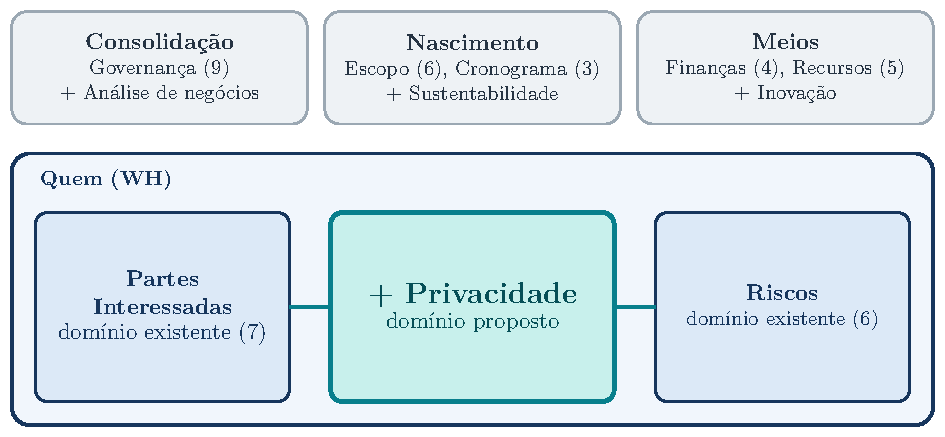
\includegraphics[width=\linewidth]{out/Fig1_PT.pdf}
\leitura{As quatro concentrações são uma organização adotada neste trabalho; \textbf{Privacidade} é a contribuição deste grupo à concentração \textbf{Quem}.}

\vspace{8mm}

\begin{caixa}{Aderência aos 6 princípios}
\corpo
\textbf{1AHV} visão integral do fluxo de dados\par\medskip
\textbf{2FOV} benefício comparado ao dano potencial\par\medskip
\textbf{3QPD} privacidade como critério verificável de qualidade\par\medskip
\textbf{4BAL} decisões e responsáveis registrados\par\medskip
\textbf{5SPA} efeitos duradouros sobre pessoas\par\medskip
\textbf{6BEC} canais para contestação e aprendizado
\end{caixa}
\end{minipage}\hfill
\begin{minipage}[t]{0.485\linewidth}
% ------------------------------ COLUNA DIREITA -------------------------------
\figtitulo{Figura 2 --- Como o domínio percorre o projeto}
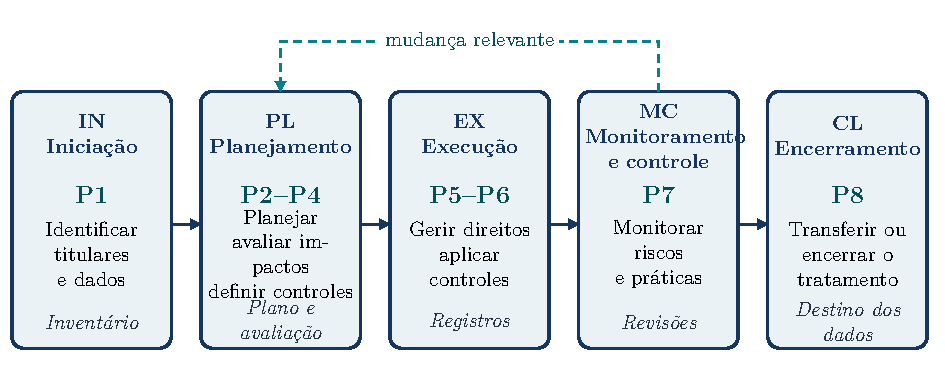
\includegraphics[width=\linewidth]{out/Fig2_PT.pdf}
\leitura{Os \textbf{P1--P8 são propostas do grupo}. A seta de retorno representa reavaliação; o tratamento de dados pode continuar após o encerramento do projeto.}

\vspace{8mm}

\figtitulo{Figura 3 --- Gêmeos digitais: a direção do fluxo define a exposição}
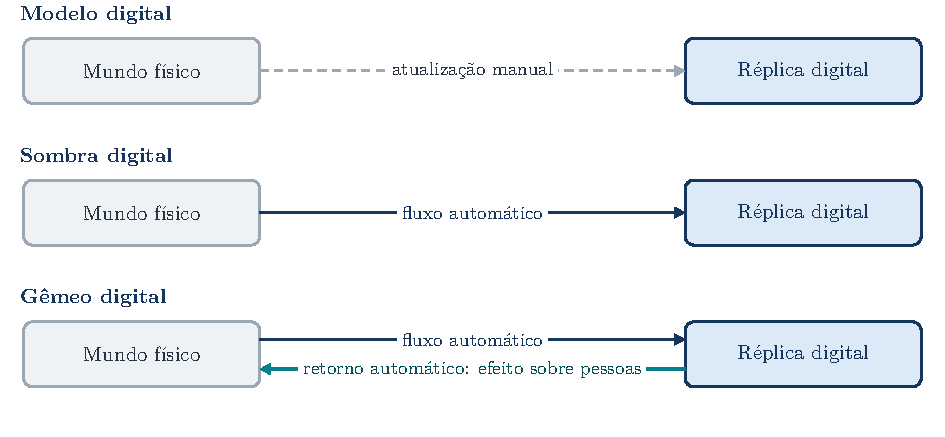
\includegraphics[width=\linewidth]{out/Fig4_PT.pdf}
\leitura{A classificação segue Kritzinger et al. [11]; quanto mais automático e frequente o fluxo, maior a exposição das pessoas. P1--P8 devem identificar titulares, finalidades, compartilhamentos, riscos e destino dos registros sem duplicar Partes Interessadas e Riscos. As inclusões propostas aos 13 processos existentes e as interfaces com as demais concentrações estão no relatório (\S7).}

\vspace{8mm}

\begin{caixa}{Referências}
\fontsize{20}{26}\selectfont
Numeração do relatório completo, em ordem alfabética.\par\smallskip
[1] ANPD. Relatório de Impacto à Proteção de Dados Pessoais (RIPD): perguntas e respostas.\par
[2] BRASIL. Lei nº 13.709/2018 (LGPD).\par
[3] BROOKS et al. NISTIR 8062, 2017.\par
[5] DHINAKARAN et al. \textit{MethodsX}, 2025.\par
[6] DTC. Digital Twin Consortium defines digital twin, 2020.\par
[7] DTC. Digital twins capabilities periodic table, v. 1.2, 2025.\par
[8] DTC. AI agent capabilities periodic table, v. 1.0, 2025.\par
[10] KORCHENKO et al. \textit{Sustainability}, 2026.\par
[11] KRITZINGER et al. \textit{IFAC-PapersOnLine}, 2018.\par
[12] NIST. Privacy Framework v. 1.0, 2020.\par
[13] PMI. \textit{PMBOK Guide}, 8. ed., 2025 (\S\S2.5 e 2.7).\par
[17] WANG et al. \textit{IEEE Internet of Things Journal}, 2023.\par\smallskip
Referências completas, com DOI e endereço, no relatório.
\end{caixa}
\end{minipage}

\end{document}
